\documentclass[a4paper,12pt]{report}

\usepackage[utf8]{inputenc}
\usepackage{amsmath}
\usepackage{graphicx}
\usepackage{hyperref}
\usepackage{geometry}
\usepackage[labelfont=bf]{caption}
\usepackage{caption}
\usepackage{subcaption}

\geometry{a4paper, margin=1in}
\setlength{\parindent}{24pt}
\begin{document}

\begin{titlepage}
    \centering
    {\large\bfseries RANCANG BANGUN SISTEM PEMBELIAN TIKET PESAWAT BERBASIS APLIKASI DESKTOP GUI DENGAN BAHASA C DAN DATABASE MYSQL\par}
    \vspace{0.3cm}
    {\large\bfseries PROJECT AKHIR\par}
    {\large\bfseries PRAKTIKUM DASAR PEMROGRAMAN\par}
    \vspace{2cm}
    \vspace*{0.5cm}
    
\includegraphics[width=0.4\textwidth]{Logo_PENS.png}\par\vspace{1cm}
    \vspace{1cm}
    {\large\bfseries Dosen :\par}
    {\Large\itshape Norma Ningsih, S.ST., M.T.\par}
    \vspace{1cm}
    {\large\bfseries Oleh :\par}
    {\Large\itshape Muqsith Barru Pamungkas - 2423600035\\Riski Gana Prasetya - 2423600053\par}
    \vspace{1cm}
    {\scshape\LARGE Teknologi Rekayasa Internet \par}
    {\scshape\LARGE Departemen Teknik Elektro \par}
    \vspace{0.5cm}
    {\scshape\Large POLITEKNIK ELEKTRONIKA NEGERI SURABAYA\par}
    {\scshape\Large 2024\par}
    \vfill
\end{titlepage}

% \title{RANCANG BANGUN SISTEM PEMBELIAN TIKET PESAWAT BERBASIS APLIKASI DESKTOP GUI DENGAN BAHASA C DAN MYSQL}
% \author{{Muqsith Barru Pamungkas}\and
% \date{\today}
% {Riski Gana Prasetya}}
% \begin{document}
% \begin{abstract}
% Makalah ini memberikan contoh sederhana bagaimana membuat dokumen menggunakan LaTeX. Kami mencakup elemen-elemen dasar seperti judul, penulis, abstrak, pendahuluan, dan kesimpulan. LaTeX adalah alat yang sangat berguna untuk penulisan dokumen ilmiah karena kemampuannya untuk mengatur format secara otomatis.
% \end{abstract}

\section{Tujuan}
\label{sec:intro}

\begin{itemize}
    \item  Merancang sistem penjualan dan pembelian tiket pesawat menggunakan bahasa c berbasis gui dengan mysql sebagai database
\end{itemize}

\section{Pendahuluan}
\subsection{Bahasa C}


\indent Bahasa C oleh Dennis M. Ritchie pada tahun 1972 di laboratorium Bell ditemukan. Pengembangan BPCL (Basic Combined Program Language) yang dibuat oleh Dr.
Martin Richard yang selanjutnya dikembangkan oleh Ken Thompson dan diseleksi dengan
Language B.Dari ketertarikan Dennis pada penerjemah bahasa B, kemudian dikembangkan menjadi
sebuah kompiler yang disebut C.
Bahasa pemrograman C merupakan sebuah bahasa pemrograman tingkat menengah yang relatif mudah untuk di pelajari, sekain bahasa yang mudah untuk di pelajari bahasa c juga memiliki kemampuan performa yang tinggi serta
bahasa c mempunyai sifat portable dalam hal ini bahasa c yang ditulis dalam satu komputer bisa dipindahkan ke komputer lain tanpa mengotak-atiknya,tanpa muncul kerumitan dalam modifikasinya. 
Dalam pengaplikasiannya bahasa C sering digunakan dalam pembuatan berbagai aplikasi seperti sistem operasi,antivirus,hingga compiler bahasa pemrograman, bahasa c ini juga merupakan induk dari beberapa bahasa seperti bahasa C++, C-Sharp, dan java.
Karena sifat bahasa c yang mudah dipahami, bahasa c menjadi bahasa pemrograman yang paling sering digunkan.
% tambahi maneh kurang okeh ketoke 

\subsection{GIMP Toolkit (GTK)}
\indent GUI atau singkatan dari Graphical User Interface yang memungkinkan pengguna untuk berinteraksi dengan perangkat keras komputer serta memudahkan dalam mengoperasikan sebuah sistem operasi (user friendly). GUI adalah sarana 
penghubug antara si pengguna(user) dengan aplikasi yang digunakan. Salah satu jenis Toolkit GUI yang populer adalah GIMP Toolkit atau GTK. 
GTK atau dikenal juga GIMP ToolKit adalah software yang digunakan untuk membangun sebuah tampilan aplikasi(GUI) lintas platform yang pertama kali dikembangkan oleh
GNU Image Manipulation Program (GIMP). ToolKit ini menyediakan berbagai macam widget yang sangat membantu dalam pembuatan aplikasi dan mampu support langsung berbagai bahasa seperti c,c++,dan pythpon
% ini juga tambahi neh seh kurang

\subsection{MySql}
% otw
\section{Tampilan Aplikasi}




Dalam bagian ini, kita menjelaskan metode yang digunakan untuk menulis makalah ini. Penulis dapat menggunakan berbagai paket dan perintah LaTeX untuk menyusun dokumen yang rapi dan terorganisir.

\section{Code Program}
Beberapa paket yang digunakan dalam dokumen ini meliputi:
\begin{itemize}
    \item \texttt{inputenc} untuk pengkodean karakter.
    \item \texttt{amsmath} untuk menulis rumus matematika.
    \item \texttt{graphicx} untuk menyisipkan gambar.
    \item \texttt{hyperref} untuk membuat hyperlink.
    \item \texttt{geometry} untuk mengatur margin halaman.
\end{itemize}

\section{Analisa}

LaTeX sangat berguna untuk menulis rumus matematika dan menyisipkan gambar. Berikut adalah contoh rumus matematika:
\begin{equation}
E = mc^2
\end{equation}

Dan berikut adalah contoh gambar yang disisipkan:
\begin{figure}[h]
    \centering
    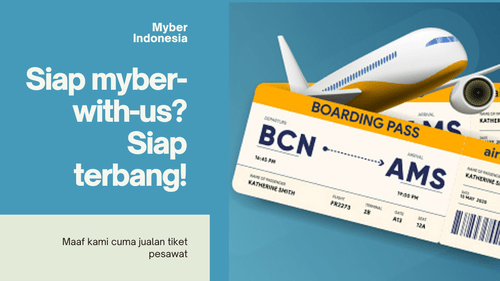
\includegraphics[width=0.5\textwidth]{../assets/banner.png}
    \caption{Contoh gambar}
    \label{fig:example}
\end{figure}



\section{Kesimpulan}
LaTeX adalah alat yang sangat berguna untuk menulis dokumen ilmiah. Dengan menggunakan LaTeX, penulis dapat dengan mudah mengatur format dokumen dan fokus pada konten.

\section*{Referensi}
\begin{itemize}
    \item Lamport, L. (1994). \textit{LaTeX: A Document Preparation System}. Addison-Wesley.
    \item \url{https://www.latex-project.org/}
\end{itemize}

\end{document}
